\begin{figure}[t]
\centering

% ---------------- Latency ----------------
\begin{subfigure}{0.49\linewidth}
\centering
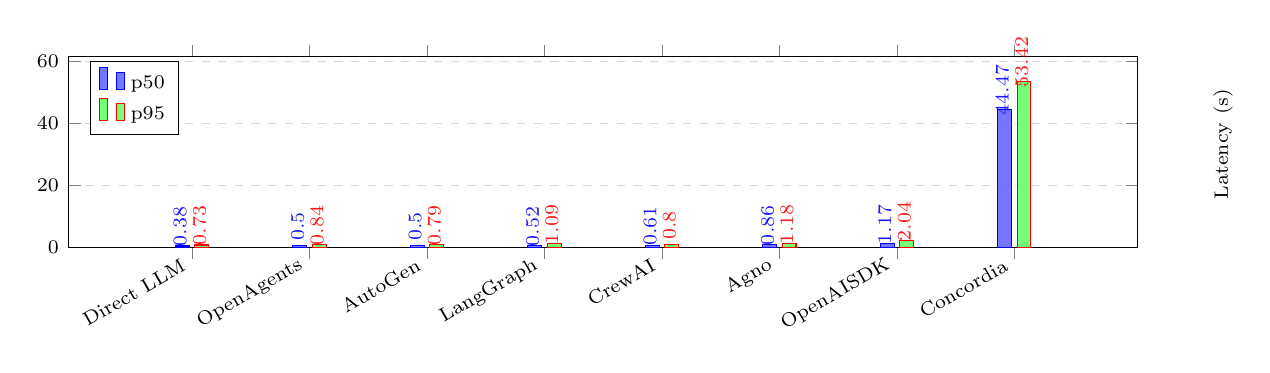
\begin{tikzpicture}
\begin{axis}[
    width=1.25\linewidth,
    height=4cm,
    ymin=0,
    ymax=61.433,
    symbolic x coords={Direct LLM,OpenAgents,AutoGen,LangGraph,CrewAI,Agno,OpenAISDK,Concordia},
    xtick=data,
    xticklabel style={rotate=30, anchor=east, font=\scriptsize},
    ylabel={Latency (s)},
    ylabel style={at={(axis description cs:1.08,0.2)}, anchor=west},
    legend style={at={(0.02,0.98)}, anchor=north west, font=\scriptsize},
    tick label style={font=\scriptsize},
    ylabel style={font=\scriptsize},
    xlabel style={font=\scriptsize},
    ybar,
    bar width=5pt,
    enlarge x limits=0.15,
    ymajorgrids=true,
    grid style={dashed,gray!30},
    nodes near coords,
    nodes near coords style={
        font=\scriptsize,
        yshift=7pt,
        xshift=5pt,
        anchor=south,
        rotate=90
    },
    every axis plot/.append style={fill opacity=0.9}
]
\addplot+[fill=blue!60] coordinates {(Direct LLM,0.379) (OpenAgents,0.495) (AutoGen,0.496) (LangGraph,0.524) (CrewAI,0.611) (Agno,0.860) (OpenAISDK,1.170) (Concordia,44.473)};
\addplot+[fill=green!60] coordinates {(Direct LLM,0.730) (OpenAgents,0.840) (AutoGen,0.787) (LangGraph,1.093) (CrewAI,0.801) (Agno,1.183) (OpenAISDK,2.036) (Concordia,53.420)};
\legend{p50, p95}
\end{axis}
\end{tikzpicture}
\caption{Latency}
\end{subfigure}
\hfill

% ---------------- Throughput ----------------
\begin{subfigure}{0.49\linewidth}
\centering
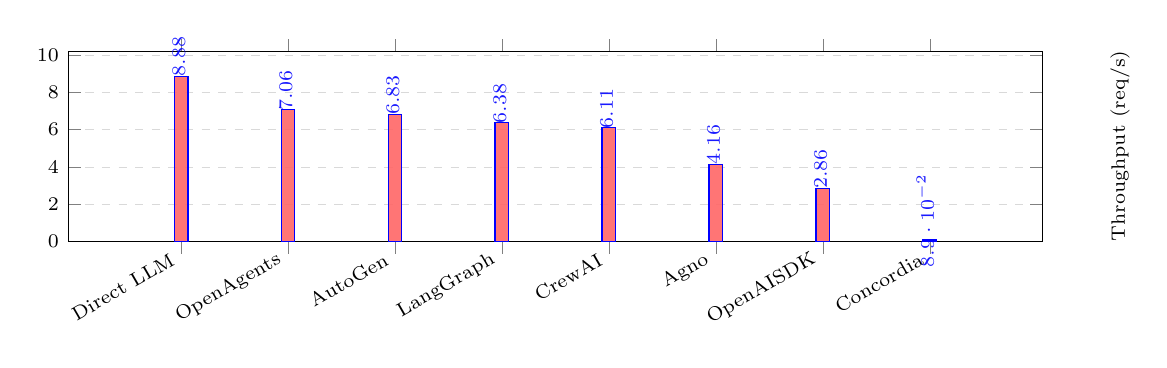
\begin{tikzpicture}
\begin{axis}[
    width=1.15\linewidth,
    height=4cm,
    ymin=0,
    ymax=10.206,
    symbolic x coords={Direct LLM,OpenAgents,AutoGen,LangGraph,CrewAI,Agno,OpenAISDK,Concordia},
    xtick=data,
    xticklabel style={rotate=30, anchor=east, font=\scriptsize},
    ylabel={Throughput (req/s)},
    ylabel style={at={(axis description cs:1.08,-0.05)}, anchor=west},
    tick label style={font=\scriptsize},
    ylabel style={font=\scriptsize},
    xlabel style={font=\scriptsize},
    ybar,
    bar width=5pt,
    enlarge x limits=0.15,
    ymajorgrids=true,
    grid style={dashed,gray!30},
    nodes near coords,
    nodes near coords style={
        font=\scriptsize,
        yshift=7pt,
        xshift=5pt,
        anchor=south,
        rotate=90
    },
    every axis plot/.append style={fill opacity=0.9}
]
\addplot+[fill=red!60] coordinates {(Direct LLM,8.875) (OpenAgents,7.062) (AutoGen,6.827) (LangGraph,6.377) (CrewAI,6.113) (Agno,4.158) (OpenAISDK,2.860) (Concordia,0.089)};
\end{axis}
\end{tikzpicture}
\caption{Throughput}
\end{subfigure}

\vspace{0.6em}

% ---------------- Mean Output ----------------
\begin{subfigure}{0.49\linewidth}
\centering
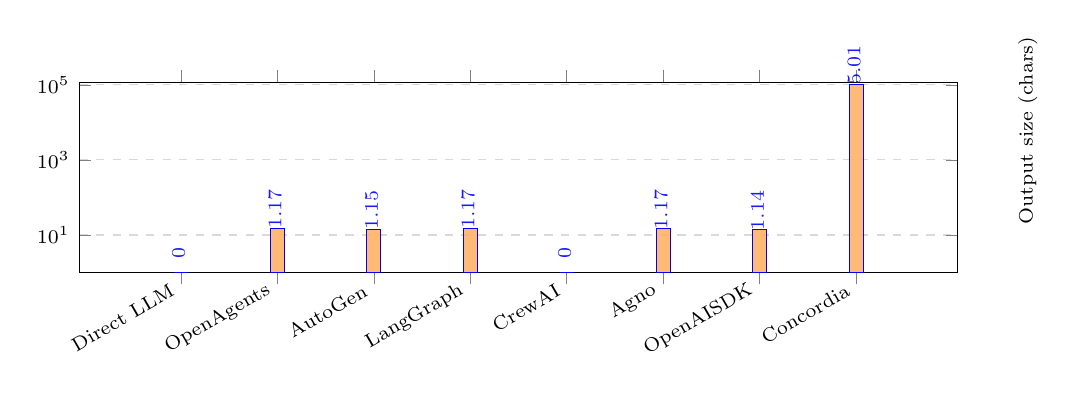
\begin{tikzpicture}
\begin{axis}[
    width=1.05\linewidth,
    height=4cm,
    ymode=log,
    log basis y=10,
    ymin=1,
    ymax=117991.564,
    symbolic x coords={Direct LLM,OpenAgents,AutoGen,LangGraph,CrewAI,Agno,OpenAISDK,Concordia},
    xtick=data,
    xticklabel style={rotate=30, anchor=east, font=\scriptsize},
    ylabel={Output size (chars)},
    ylabel style={at={(axis description cs:1.08,0.2)}, anchor=west},
    tick label style={font=\scriptsize},
    ylabel style={font=\scriptsize},
    xlabel style={font=\scriptsize},
    ybar,
    bar width=5pt,
    enlarge x limits=0.15,
    ymajorgrids=true,
    grid style={dashed,gray!30},
    nodes near coords,
    nodes near coords style={
        font=\scriptsize,
        yshift=7pt,
        xshift=5pt,
        anchor=south,
        rotate=90
    },
    every axis plot/.append style={fill opacity=0.9}
]
\addplot+[fill=orange!60] coordinates {(Direct LLM,1.000) (OpenAgents,14.900) (AutoGen,14.220) (LangGraph,14.900) (CrewAI,1.000) (Agno,14.800) (OpenAISDK,13.880) (Concordia,102601.360)};
\end{axis}
\end{tikzpicture}
\caption{Mean output}
\end{subfigure}
\hfill

% ---------------- Output Summary ----------------
\begin{subfigure}{0.49\linewidth}
\centering
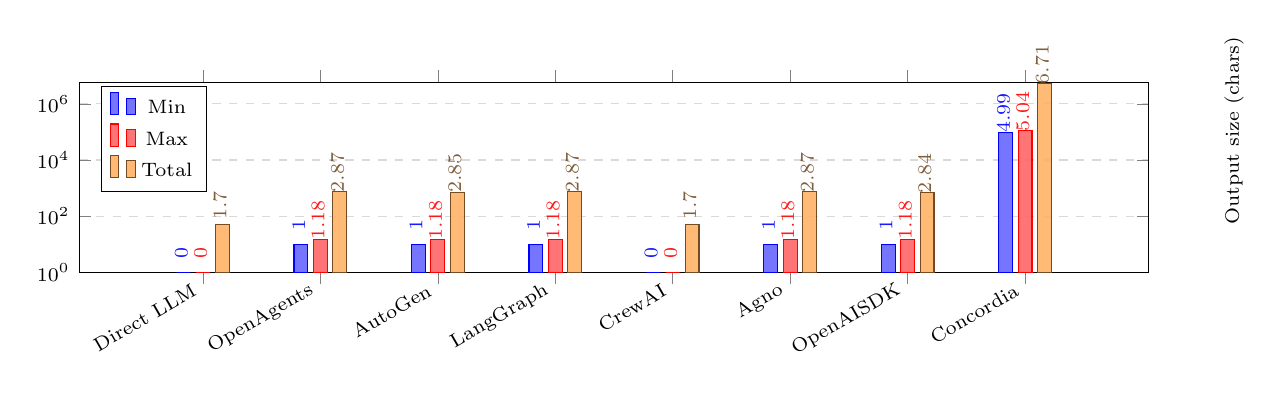
\begin{tikzpicture}
\begin{axis}[
    width=1.25\linewidth,
    height=4cm,
    ymode=log,
    log basis y=10,
    ymin=1,
    ymax=5899578.200,
    symbolic x coords={Direct LLM,OpenAgents,AutoGen,LangGraph,CrewAI,Agno,OpenAISDK,Concordia},
    xtick=data,
    xticklabel style={rotate=30, anchor=east, font=\scriptsize},
    ylabel={Output size (chars)},
    ylabel style={at={(axis description cs:1.08,0.2)}, anchor=west},
    legend style={at={(0.02,0.98)}, anchor=north west, font=\scriptsize},
    tick label style={font=\scriptsize},
    ylabel style={font=\scriptsize},
    xlabel style={font=\scriptsize},
    ybar,
    bar width=5pt,
    enlarge x limits=0.15,
    ymajorgrids=true,
    grid style={dashed,gray!30},
    nodes near coords,
    nodes near coords style={
        font=\scriptsize,
        yshift=7pt,
        xshift=5pt,
        anchor=south,
        rotate=90
    },
    every axis plot/.append style={fill opacity=0.9}
]
\addplot+[fill=blue!60] coordinates {(Direct LLM,1.000) (OpenAgents,10.000) (AutoGen,10.000) (LangGraph,10.000) (CrewAI,1.000) (Agno,10.000) (OpenAISDK,10.000) (Concordia,97448.000)};
\addplot+[fill=red!60] coordinates {(Direct LLM,1.000) (OpenAgents,15.000) (AutoGen,15.000) (LangGraph,15.000) (CrewAI,1.000) (Agno,15.000) (OpenAISDK,15.000) (Concordia,110886.000)};
\addplot+[fill=orange!60] coordinates {(Direct LLM,50.000) (OpenAgents,745.000) (AutoGen,711.000) (LangGraph,745.000) (CrewAI,50.000) (Agno,740.000) (OpenAISDK,694.000) (Concordia,5130068.000)};
\legend{Min, Max, Total}
\end{axis}
\end{tikzpicture}
\caption{Output summary}
\end{subfigure}

\caption{Framework overhead results for 50 trials of the trivial task (``What is 2+2?''). 
Frameworks are ordered by increasing p50 latency.
\textbf{Direct LLM}, \textbf{OpenAgents}, \textbf{AutoGen}, \textbf{LangGraph}, \textbf{CrewAI}, \textbf{Agno}, \textbf{OpenAISDK}, \textbf{Concordia}.}
\label{fig:framework-overhead}
\end{figure}